\section{Results}
\label{sec:results}

\subsection{Part 1}

Table~\ref{tab:p1models} compares the reason-labeling methods. The unsupervised
mixture used on its own is clearly the weakest entry (0.780 / 0.570), and
one-vs-rest logistic regression---the obvious supervised default---is beaten by
the balanced multinomial formulation. Self-training adds the largest single
increment, and folding the mixture posterior into the pseudo-labeling step gives
the best validation sample-F1 and the best cross-validated macro-F1 of any
configuration we tried.

\begin{table}[t]
\centering\small
\setlength{\tabcolsep}{4pt}
\begin{tabular}{lcccc}
\toprule
& \multicolumn{2}{c}{Validation} & \multicolumn{2}{c}{Repeated CV} \\
\cmidrule(lr){2-3}\cmidrule(lr){4-5}
Model & samp.\ F1 & macro F1 & samp.\ F1 & macro F1 \\
\midrule
One-vs-rest LR ($C{=}1$)        & 0.868 & 0.706 & 0.898 & 0.797 \\
$k$NN cosine ($k{=}10$)         & 0.872 & 0.607 & 0.881 & 0.734 \\
GMM-30 cluster-then-label       & 0.780 & 0.570 & 0.819 & 0.640 \\
Multinomial LR, unbalanced      & 0.850 & 0.677 & 0.894 & 0.765 \\
Balanced mult.\ LR $+$ $k$NN    & 0.885 & 0.724 & 0.898 & 0.800 \\
Self-training, no GMM           & 0.889 & 0.723 & 0.913 & 0.805 \\
\textbf{Final: GMM self-train.} & \textbf{0.893} & 0.714 & \textbf{0.914} & \textbf{0.814} \\
\bottomrule
\end{tabular}
\caption{Part~1 model comparison. Validation is the 78 labeled trials; repeated CV
is 8 repeats of 5-fold CV over all 235 labeled trials.}
\label{tab:p1models}
\end{table}

Table~\ref{tab:p1ablation} adds each optional feature block to the final model.
Every block leaves validation sample-F1 unchanged or worse, and no block moves
cross-validated macro-F1 by more than 0.013 in either direction; we therefore
submit the embeddings-only model. Section~\ref{sec:discussion} explains why.

\begin{table}[t]
\centering\small
\setlength{\tabcolsep}{4pt}
\begin{tabular}{lcccc}
\toprule
& \multicolumn{2}{c}{Validation} & \multicolumn{2}{c}{Repeated CV} \\
\cmidrule(lr){2-3}\cmidrule(lr){4-5}
Feature set & samp.\ F1 & macro F1 & samp.\ F1 & macro F1 \\
\midrule
\textbf{Embeddings only}          & \textbf{0.893} & \textbf{0.714} & 0.914 & 0.814 \\
$+$ \texttt{start\_year}          & 0.891 & 0.711 & 0.912 & 0.807 \\
$+$ criteria TF-IDF (SVD 50)      & 0.876 & 0.709 & 0.913 & 0.801 \\
$+$ diseases TF-IDF (SVD 20)      & 0.876 & 0.696 & 0.914 & 0.806 \\
$+$ Morgan fingerprints (SVD 20)  & 0.889 & 0.719 & 0.918 & 0.815 \\
\bottomrule
\end{tabular}
\caption{Part~1 feature ablation, final model. Extra blocks never improve
validation sample-F1.}
\label{tab:p1ablation}
\end{table}

Per-label validation F1 for the final model is Safety 0.947, Funding 0.400,
Efficacy 0.741, Recruitment 0.980 and Other 0.500, giving sample-F1 0.893 and
macro-F1 0.714. Trained on the 157 labeled trials it admitted 985 pseudo-labels;
refit on all 235 labeled trials it scores \textbf{0.89423} sample-F1 on the Kaggle
test set \TODO{confirm against leaderboard}. Figure~\ref{fig:p1freq} shows the
predicted reason frequencies: relative to the labeled trials the model assigns
more Safety (0.173 vs.\ 0.106) and less Recruitment (0.587 vs.\ 0.643) to the
later test trials, the direction of drift the task description predicts.

\begin{figure}[t]
\centering
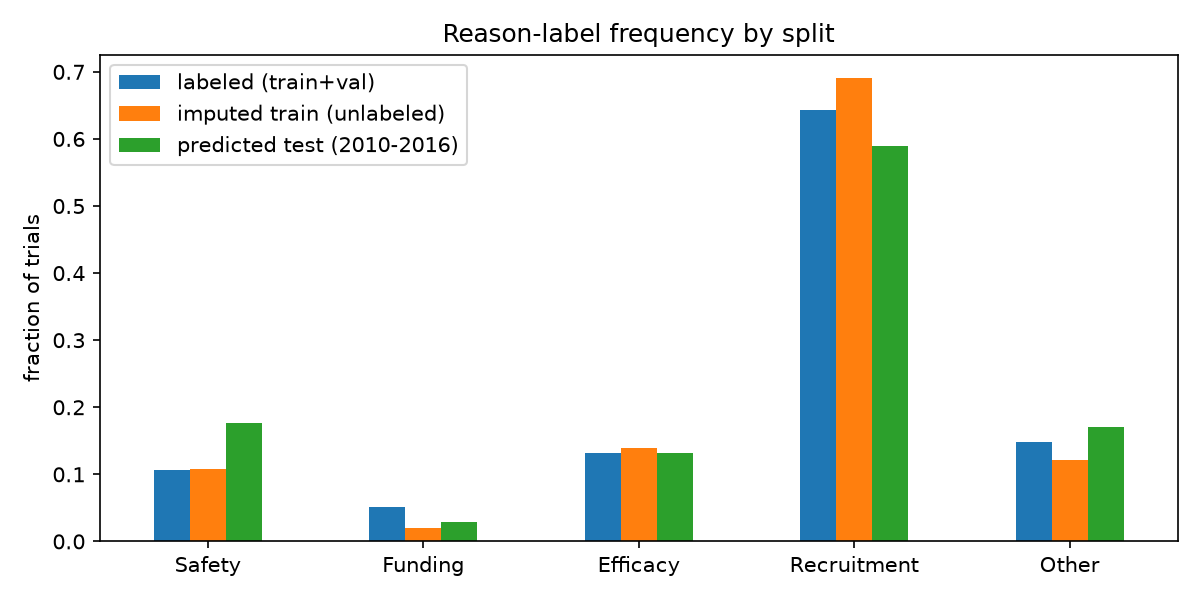
\includegraphics[width=0.95\linewidth]{part1_label_frequency.png}
\caption{Reason-label frequency across the labeled trials, the imputed unlabeled
training trials, and the predicted 2010--2016 test trials.}
\label{fig:p1freq}
\end{figure}

\subsection{Part 2}

Table~\ref{tab:p2val} reports per-phase validation metrics. Multinomial naive
Bayes separates classes about as well as logistic regression on ROC-AUC but is
wildly overconfident, so its log loss (2.646) is unusable for a log-loss
competition. The stack improves log loss and PR-AUC in every phase; adding
recency weights improves log loss further and recovers the F1 that the unweighted
stack gave up.

\begin{table}[t]
\centering\small
\setlength{\tabcolsep}{4pt}
\begin{tabular}{llcccc}
\toprule
Model & Phase & F1 & ROC-AUC & PR-AUC & log loss \\
\midrule
\multirow{4}{*}{MNB (per phase)}
 & I    & 0.737 & 0.717 & 0.733 & 2.684 \\
 & II   & 0.645 & 0.694 & 0.623 & 2.945 \\
 & III  & 0.796 & 0.699 & 0.783 & 2.308 \\
 & mean & 0.726 & 0.703 & 0.713 & 2.646 \\
\midrule
\multirow{4}{*}{Baseline LR (per phase)}
 & I    & 0.774 & 0.780 & 0.809 & 0.609 \\
 & II   & 0.631 & 0.729 & 0.711 & 0.610 \\
 & III  & 0.813 & 0.764 & 0.868 & 0.553 \\
 & mean & 0.739 & 0.758 & 0.796 & 0.591 \\
\midrule
\multirow{4}{*}{Improved: stacked}
 & I    & 0.730 & 0.772 & 0.816 & 0.570 \\
 & II   & 0.661 & 0.749 & 0.733 & 0.591 \\
 & III  & 0.817 & 0.787 & 0.883 & 0.516 \\
 & mean & 0.736 & 0.769 & 0.810 & 0.559 \\
\midrule
\multirow{4}{*}{\textbf{Final: $+$ recency ($\tau{=}3$)}}
 & I    & 0.793 & 0.793 & 0.828 & 0.557 \\
 & II   & 0.648 & 0.754 & 0.735 & 0.593 \\
 & III  & 0.824 & 0.787 & 0.881 & 0.518 \\
 & mean & \textbf{0.755} & \textbf{0.778} & \textbf{0.814} & \textbf{0.556} \\
\bottomrule
\end{tabular}
\caption{Part~2 validation metrics by phase. F1 uses a 0.5 threshold; ROC-AUC,
PR-AUC and log loss use predicted probabilities, with $\text{label}=1$ positive.}
\label{tab:p2val}
\end{table}

The time-based holdouts (Table~\ref{tab:p2holdout}) confirm the ordering under the
distribution shift that actually matters. Fitting on trials up to 2009 and scoring
2010--2013, the stack cuts log loss from 0.5879 to 0.5514 and recency weighting
takes it to 0.5475; on the harder 2012--2013 holdout the margin widens (0.5192
$\to$ 0.4657 $\to$ 0.4553).

\begin{table}[t]
\centering\small
\setlength{\tabcolsep}{4pt}
\begin{tabular}{llcccc}
\toprule
Holdout & Model & F1 & ROC-AUC & PR-AUC & log loss \\
\midrule
\multirow{4}{*}{fit $\leq$ 2009}
 & MNB       & 0.8083 & 0.6295 & 0.7301 & 2.4794 \\
 & Base.\ LR & 0.8051 & 0.6943 & 0.7847 & 0.5879 \\
 & Stacked   & 0.8090 & 0.7248 & 0.8183 & 0.5514 \\
 & $+$ rec.  & \textbf{0.8094} & \textbf{0.7311} & \textbf{0.8205} & \textbf{0.5475} \\
\midrule
\multirow{4}{*}{fit $\leq$ 2011}
 & MNB       & 0.8576 & 0.5970 & 0.7740 & 2.0120 \\
 & Base.\ LR & 0.8654 & 0.7042 & 0.8290 & 0.5192 \\
 & Stacked   & 0.8697 & 0.7539 & 0.8850 & 0.4657 \\
 & $+$ rec.  & \textbf{0.8758} & \textbf{0.7604} & \textbf{0.8865} & \textbf{0.4553} \\
\bottomrule
\end{tabular}
\caption{Part~2 time-based holdouts, mean over phases. The 2009 cut is evaluated
on 2010--2013 and the 2011 cut on 2012--2013. These mimic the later start years of
the test set and were used to select $\tau$.}
\label{tab:p2holdout}
\end{table}

On the Kaggle test set the final submission scores \textbf{0.58688} mean log loss
\TODO{confirm against leaderboard}, against 0.556 on validation---a gap we return
to in Section~\ref{sec:discussion}.

\subsection{Error analysis across reason categories}

Table~\ref{tab:p2errors} and Figure~\ref{fig:p2err} break the failed validation
trials down by phase and stopping reason. Two patterns are robust. First, error
rates are much higher in Phase~III (0.57--1.00 for the baseline) than in Phase~II
(0.00--0.38), despite Phase~III having more training data. Second, the largest and
therefore most trustworthy groups---Phase~II Recruitment ($n{=}87$) and the three
no-recorded-reason groups ($n{=}28/144/82$)---all improve monotonically from
baseline to stack to recency-weighted stack; the Phase~I no-reason group falls
from 0.643 to 0.321.

\begin{figure*}[t]
\centering
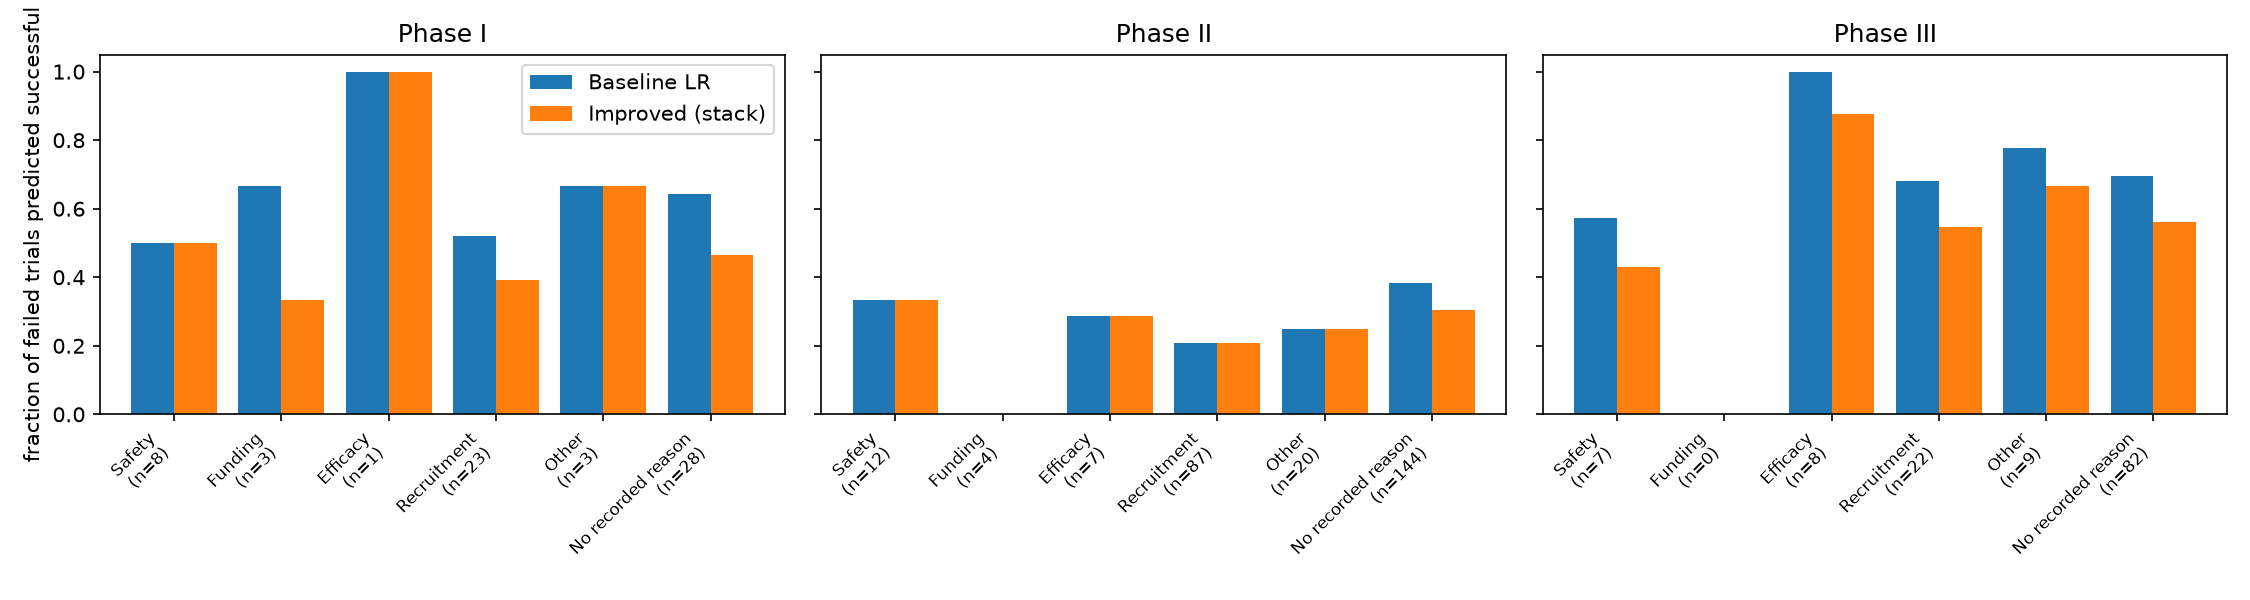
\includegraphics[width=\textwidth]{part2_error_by_reason.png}
\caption{Fraction of failed validation trials incorrectly predicted successful,
by phase and stopping reason, for the criteria-only baseline and the stacked
ensemble. Group sizes are given in the tick labels.}
\label{fig:p2err}
\end{figure*}

\begin{table*}[t]
\centering\small
\begin{tabular}{llccccccc}
\toprule
& & \multicolumn{3}{c}{Group composition} & & \multicolumn{3}{c}{Fraction predicted successful} \\
\cmidrule(lr){3-5}\cmidrule(lr){7-9}
Phase & Reason & $n$ trials & $n$ true & $n$ predicted & & Baseline LR & Improved & Final \\
\midrule
I & Safety             &  8 &  1 &  7 & &  0.500 & 0.500 & 0.375 \\
I & Funding            &  3 &  1 &  2 & &  0.667 & 0.333 & 0.000 \\
I & Efficacy           &  1 &  0 &  1 & &  1.000 & 1.000 & 0.000 \\
I & Recruitment        & 23 &  2 & 21 & &  0.522 & 0.391 & 0.174 \\
I & Other              &  3 &  0 &  3 & &  0.667 & 0.667 & 0.667 \\
I & No recorded reason & 28 &  0 &  0 & &  0.643 & 0.464 & 0.321 \\
\midrule
II & Safety             &  12 &  1 & 11 & & 0.333 & 0.333 & 0.250 \\
II & Funding            &   4 &  1 &  3 & & 0.000 & 0.000 & 0.000 \\
II & Efficacy           &   7 &  0 &  7 & & 0.286 & 0.286 & 0.286 \\
II & Recruitment        &  87 & 12 & 75 & & 0.207 & 0.207 & 0.149 \\
II & Other              &  20 &  3 & 17 & & 0.250 & 0.250 & 0.250 \\
II & No recorded reason & 144 &  0 &  0 & & 0.382 & 0.306 & 0.250 \\
\midrule
III & Safety             &  7 & 1 &  6 & & 0.571 & 0.429 & 0.429 \\
III & Funding            &  0 & 0 &  0 & & ---   & ---   & ---   \\
III & Efficacy           &  8 & 0 &  8 & & 1.000 & 0.875 & 1.000 \\
III & Recruitment        & 22 & 5 & 17 & & 0.682 & 0.545 & 0.455 \\
III & Other              &  9 & 2 &  7 & & 0.778 & 0.667 & 0.556 \\
III & No recorded reason & 82 & 0 &  0 & & 0.695 & 0.561 & 0.585 \\
\bottomrule
\end{tabular}
\caption{Error rates on the 452 failed validation trials, by phase and stopping
reason. ``$n$ true'' counts trials whose reason labels are ground truth from
Part~1; ``$n$ predicted'' counts trials whose reason labels are Part~1 model
predictions. A trial with several reasons appears in each of its reason rows, so
columns do not sum to the phase total.}
\label{tab:p2errors}
\end{table*}
